PanDA is a Workload Management System (WMS) %~\cite{marco2009glite} 
designed to support the execution of distributed workloads and workflows via
pilots~\cite{turilli2015comprehensive}. Pilot-capable WMS enable high
throughput execution of tasks via multi-level scheduling while supporting
interoperability across multiple sites. This is particularly relevant for LHC
experiments, where millions of tasks are executed across multiple sites every
month, analyzing and producing petabytes of data. 
% The design of PanDA WMS started in 2005 to support ATLAS\@. PanDA went into
% production for the LHC Run 1 on 2009, and was then extended with new
% subsystems for Run 2 in 2015.


% ---------------------------------------------------------------------------
% \subsection{Design}
% \label{ssec:panda_design}

% PanDA's application model assumes tasks grouped into workloads and
% workflows. Tasks represent a set of operations performed on data sets
% stored in one or more input files. Tasks are decomposed into jobs, where
% each job consists of the task's operations performed on a partition of the
% task's data set. Since 2005, a certain amount of parallelism has been
% progressively introduced for job execution~\cite{crooks2012multi} but, so
% far, HEP applications have not required a message passing interface (MPI).

% PanDA's usage model assumes multitenancy of resources and at least two
% types of HEP users: individual researchers and groups executing so called
% `production' workflows. PanDA's security model is based on separation
% between authentication, authorization and accounting for both single users
% and group of users. Both authentication and authorization are based on
% digital certificates and on the virtual organization
% abstraction~\cite{foster2001anatomy}.

% Currently, PanDA's execution model is based on four main abstractions:
% task, job, queue, and pilot. Both tasks and jobs are assumed to have
% attributes and states and to be queued into a global queue for execution.
% Prioritization and binding of jobs are assumed to depend on the attributes
% of each job. Pilot is used to indicate the abstraction of resource
% capabilities. Each job is thought to be bound to one pilot and executed on
% the site where the pilot has been instantiated.

% In PanDA's data model, each datum refers to the recorded or simulated
% measurement of a physical process. Data can be packaged into files or other
% containers. As with jobs, data have both attributes and states, and some of
% the attributes are shared between events and jobs. Raw, reconstruction, and
% simulation data are assumed to be distributed across multiple storage
% facilities and managed by the ATLAS Distributed Data Management
% (DDM)%~\cite{garonne2012atlas}. 
% When necessary, datasets required by each job are assumed to be replicated
% over the network, both for input and output data.

% PanDA's design supports provenance and traceability for both jobs and data.
% Attributes enable provenance by linking jobs and data items, providing
% information like ownership or project affiliation. States enable
% traceability by providing information about the stage of the execution in
% which each job or data item is or has been.

% ---------------------------------------------------------------------------
% \subsection{Implementation and Execution}
% \label{ssec:panda_arch}

The implementation of PanDA WMS consists of several interconnected
subsystems,
% , most of them built from off-the-shelf and Open Source components.
% Subsystems communicate 
communicating via dedicated API or HTTP messaging, and implemented by one or
more modules. Databases are used to store eventful entities like tasks, jobs
and input/output data, and to store information about sites, resources,
logs, and accounting.

Currently, PanDA's architecture has five main subsystems: PanDA
Server~\cite{maeno2011overview},
AutoPyFactory~\cite{caballero2012autopyfactory}, PanDA
Pilot~\cite{nilsson2011atlas}, JEDI~\cite{borodin2015scaling}, and PanDA
Monitoring~\cite{klimentov2011atlas}. Other subsystems are used by some of
ATLAS workflows % (e.g., PanDA Event Service~\cite{calafiura2015atlas}), 
but we do not discuss them as they are not relevant to an understanding of
how PanDA has been ported to supercomputers. For a full list of subsystems
see Ref.~\cite{panda-wiki_url}. Fig.~\ref{fig:architecture} shows a
diagrammatic representation of PanDA main subsystems, highlighting the
execution process of tasks while omitting monitoring details to improve
readability.

% During LHC Run 1, PanDA required users to perform a static conversion
% between tasks and jobs: tasks were described as a set of jobs and then
% submitted to the PanDA Server. This introduced inefficiency both with
% usability and resource utilization.%~\cite{borodin2015unified}. Ideally,
% users should conceive analyses in terms of one or more, possibly related
% tasks, while the execution manager (i.e., PanDA) should partition tasks
% into jobs, depending on execution constraints. Further, due to the static
% partitioning of tasks into jobs, PanDA instantiates pilots on sites without
% taking into account the heterogeneity and dynamicity of the resources. An
% optimal sizing of each job should take into account these properties.

% Another problem of static job sizing is that PanDA instantiates pilots on
% sites with different type of resources and different models of availability
% of those resources. An optimal sizing of each job should take into account
% these properties. For example, sites may offer cores with different speed,
% networking with different amount of bandwidth, and resources could be
% guaranteed to be available for a defined amount of time or could disappear
% at any point in time as it happens with opportunistic models of resource
% provision.

% JEDI was deployed for the LHC Run 2 to address these inefficiencies. 
Users submit task descriptions to JEDI (Fig.~\ref{fig:architecture}:1) that
stores them into a queue implemented by a database
(Fig.~\ref{fig:architecture}:2). Tasks are partitioned into jobs of different
size, depending on both static and dynamic information about available
resources (Fig.~\ref{fig:architecture}:3). Jobs are bound to sites with
resources that best match jobs' requirements, and submitted to the PanDA
Server for execution (Fig.~\ref{fig:architecture}:4).

Once submitted to the PanDA Server, jobs are stored by the Task Buffer
component into a global queue implemented as a database
(Fig.~\ref{fig:architecture}:5). When jobs are submitted directly to the
PanDA Server, the Brokerage component is used to bind jobs to available
sites, depending on static information about the resources available for each
site. Jobs submitted by JEDI are already bound to sites so no further
brokerage is needed.

Once jobs are bound to sites, the Brokerage module communicates to the Data
Service module what data sets need to be made available on what site
(Fig.~\ref{fig:architecture}:6). The Data Service communicates these
requirements to the ATLAS DDM (Fig.~\ref{fig:architecture}:7) that, when
needed, replicates data sets on the required sites
(Fig.~\ref{fig:architecture}:8).

Meanwhile, AutoPyFactory defines PanDA Pilots, submitting them to a Condor-G
agent (Fig.~\ref{fig:architecture}:9). Condor-G schedules these pilots
wrapped as jobs to the required sites
(Fig.~\ref{fig:architecture}:10).

When a PanDA Pilot becomes available, it requests the Job Dispatcher module
of the PanDA Server for a job to execute (Fig.~\ref{fig:architecture}:11).
The Job Dispatcher interrogates the Task Buffer module for a job that is
bound to the site of that pilot and ready to be executed. Task Buffer checks
the global queue (i.e., the PanDA database) and, upon availability, returns a
job to the Job Dispatcher. The Job Dispatcher dispatches that job to the
PanDA Pilot (Fig.~\ref{fig:architecture}:12).

A PanDA Pilot starts a monitoring process on receiving a job and forks a
subprocess to execute the job's payload. Input data are transferred
from the stage-in location (Fig.~\ref{fig:architecture}:13), the job's
payload is executed (Fig.~\ref{fig:architecture}:14) and once completed, output
is transferred to the staging-out location (Fig.~\ref{fig:architecture}:15).

The Data Service module of the PanDA Server tracks and collects the output
generated by each job (Fig.~\ref{fig:architecture}:16), updating jobs'
attributes via the Task Buffer module (Fig.~\ref{fig:architecture}:17). When
the output of all the jobs of a task are retrieved, it is made available to
the user via PanDA Server. When a task is submitted to JEDI, task is instead
marked as done (Fig.~\ref{fig:architecture}:18) and the result of its
execution is made available to the user by JEDI
(Fig.~\ref{fig:architecture}:19).

\begin{figure}
    \centering
    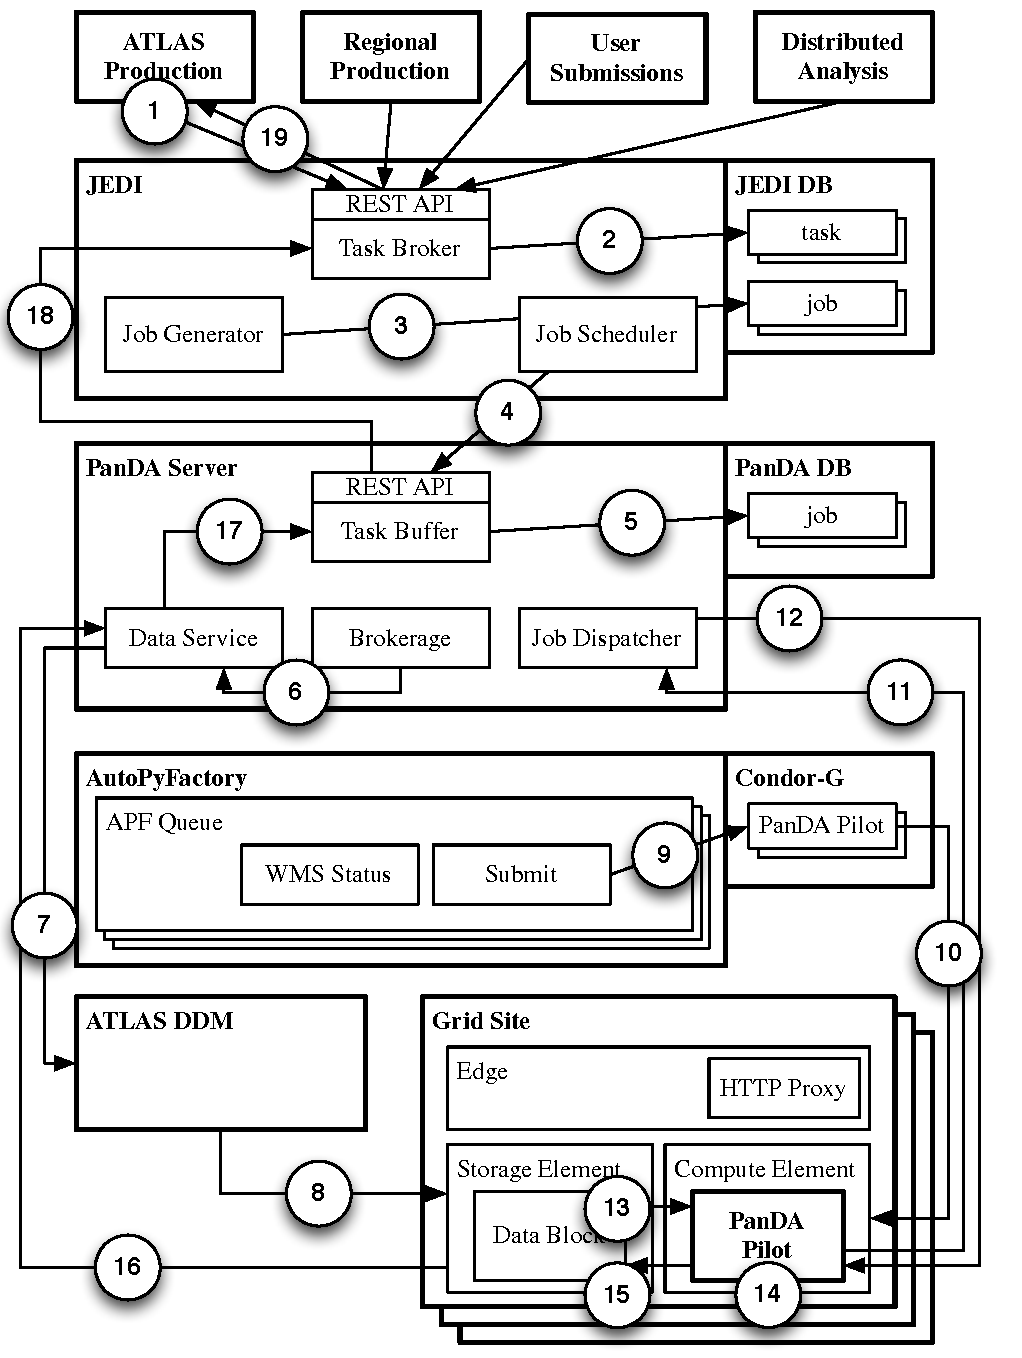
\includegraphics[width=\columnwidth]{figures/panda_architecture.pdf}
    \vspace{-0.3in}
    \caption{PanDA WMS architecture. Numbers indicates the JEDI-based
    execution process. Several subsystems, components, and architectural and
    communication details are abstracted to improve clarity.}
\label{fig:architecture}
\end{figure}